%!Tex Root = ../main.tex
% ./Packete.tex
% ./Design.tex
% ./Deklarationen.tex
% ./Vorbereitung.tex
% ./Aufgabe1.tex
% ./Aufgabe2.tex
% ./Aufgabe4.tex
% ./Appendix.tex

\section{Aufgabe 3}

\setcounter{exercise}{1}

\begin{frame}[allowframebreaks]{Aufgabe \thesection}{XOR, Quine-McCluskey, Primimplikanten, Tiefe}
  \begin{solutionnoinc}
    \begin{itemize}
      \item \alert{Minterme:} $x_{1}^{\prime}x_{2}^{\prime}x_{3},\ x_{1}^{\prime}x_{2}x_{3}^{\prime},\ x_{1}x_{2}^{\prime}x_{3}^{\prime},\ x_{1}x_{2}x_{3}$
      \item \alert{Quine-McCluskey:}
        \begin{table}
        \centering
        \begin{tblr}{
          cells = {c, white},
          row{1} = {PrimaryColor,fg=white},
          hline{2,5} = {1}{},
        }
        $L_{0}^{x_1, x_2, x_3}$ \\
        001                     \\
        010                     \\
        100                     \\
        111                     
        \end{tblr}
        \end{table}
        \begin{itemize}
          \item $Prim(xor_3) = \empty$
          \item Es gibt keine Kombinationsmöglichkeiten der Minterme aus $L_0$. Daher sind alle $L_1$-Mengen leer und die Primmenge im nächsten Schritt enthält alle vier Minterme. Der Grund ist, dass sich alle Minterme in (mindestens) zwei Literalen unterscheiden, d.h. alle Minterme sind Primimplikanten.
        \end{itemize}
    \end{itemize}
  \end{solutionnoinc}
  \begin{solution}
    \begin{table}
      \centering
      \begin{tblr}{
        cells = {c, white},
        row{1} = {PrimaryColor, fg=white},
        cell{2}{1} = {PrimaryColor, fg=white},
        cell{3}{1} = {PrimaryColor, fg=white},
        cell{4}{1} = {PrimaryColor, fg=white},
        cell{5}{1} = {PrimaryColor, fg=white},
      }
                    & 1 & 2 & 4 & 7 \\
      $x_1'x_2'x_3$ & 1 &   &   &   \\
      $x_1'x_2x_3'$ &   & 1 &   &   \\
      $x_1x_2'x_3'$ &   &   & 1 &   \\
      $x_1x_2x_3$   &   &   &   & 1
      \end{tblr}
    \end{table}
    \begin{itemize}
      \item Es ist direkt ersichtlich, dass alle Primimplikanten wesentlich sind (Regel 1). Die Disjunktion aller Minterme ist also das einzige Minimalpolynom für $xor_3$
    \end{itemize}
  \end{solution}
  \begin{solution}
    \begin{itemize}
      \item $\displaystyle \bigvee_{\mathclap{\substack{(b_1,\ldots,b_n)\in \mathbb{B}^n\\ mit \sum^n_{i=1} ungerade}}} (x_1^{b_1}\wedge \ldots \wedge x_n^{b_n}), \mathrm{wobei}\;x_{i}^{0}:=x_{i}^{\prime}\;\mathrm{und}\;x_{i}^{1}:=x_{i}$
      \item Der angegebene Ausdruck ist die Disjunktion aller Minterme für $xor_n$. In Aufgabenteil a) haben wir schon gesehen, dass alle Minterme wesentlich sind um $xor_n$ darzustellen, da weder durch Quine-McCluskey noch Primimplikantentafel Reduktionen erreicht werden können. Deswegen beschreibt auch hier die Disjunktion der Minterme das Minimalpolynom. Es sind $2^{n-1}$ Primimplikanten, je mit Länge $n$.
    \end{itemize}
  \end{solution}
  \begin{requirementsnoinc}
    \begin{itemize}
      \item $x o r_{n}(x_{1},...,x_{n})=g(x o r_{i}(x_{1},...,x_{i}),x o r_{n-i}(x_{i+1},...,x_{n})){\mathrm{~für~1}}\leq i\leq n-1$
    \end{itemize}
  \end{requirementsnoinc}
  \begin{solutionnoinc}
    \begin{itemize}
      \item Sei $b_{1}:=x o r_{i}(x_{1},...,x_{i}),~~b_{2}:=x o r_{n-i}(x_{i+1},...,x_{n})$
      \begin{enumerate}
        \item Fall $b_1 = 0$, $b_2 = 0$:\\[-0.05cm] 
          Dann ist $\displaystyle\sum_{j=1}^{i} x_j$ gerade, $\displaystyle\sum_{j=i+1}^{n} x_j$ gerade $\displaystyle\Rightarrow \sum_{j=1}^{n} x_j$ gerade $\Rightarrow g(0, 0) = 0 = xor_2(0, 0)$ 
        \item Fall $b_1 = 1$, $b_2 = 0$:\\[-0.05cm]
          Dann ist $\displaystyle\sum_{j=1}^{i} x_j$ ungerade, $\displaystyle\sum_{j=i+1}^{n} x_j$ gerade $\displaystyle\Rightarrow \sum_{j=1}^{n} x_j$ ungerade $\Rightarrow g(1, 0) = 1 = xor_2(1, 0)$ 
        \item Fall $b_0 = 1$, $b_2 = 1$:\\[-0.05cm]
          Dann ist $\displaystyle\sum_{j=1}^{i} x_j$ gerade, $\displaystyle\sum_{j=i+1}^{n} x_j$ ungerade $\displaystyle\Rightarrow \sum_{j=1}^{n} x_j$ ungerade $\Rightarrow g(0, 1) = 1 = xor_2(0, 1)$ 
        \item Fall $b_0 = 1$, $b_2 = 1$:\\[-0.05cm]
          Dann ist $\displaystyle\sum_{j=1}^{i} x_j$ ungerade, $\displaystyle\sum_{j=i+1}^{n} x_j$ ungerade $\displaystyle\Rightarrow \sum_{j=1}^{n} x_j$ gerade $\Rightarrow g(1, 1) = 1 = xor_2(1, 1)$ 
      \end{enumerate}
    \end{itemize}
  \end{solutionnoinc}
  \begin{solution}
    \begin{itemize}
      \item \alert{Zusammengefasst:}\\
        \begin{table}
          \centering
          \begin{tblr}{
            cells = {white, c},
            row{1} = {PrimaryColor,fg=white},
            vline{3} = {-}{},
          }
          $b_1$ & $b_2$ & $g$ \\
          0     & 0     & 0   \\
          0     & 1     & 1   \\
          1     & 0     & 1   \\
          1     & 1     & 0   
          \end{tblr}
        \end{table}
        $\Rightarrow g = xor_2$, also $x o r_{n}\left(x_{1},...,x_{n}\right)=x o r_{2}\left(x o r_{i}\left(x_{1},...,x_{i}\right),x o r_{n-i}\left(x_{i+1},...,x_{n}\right)\right){\mathrm{~für~1}}\leq i\leq n-1$
    \end{itemize}
  \end{solution}
  \begin{solution}
    \begin{itemize}
      \item Ein balancierter Baum hat die geringste Tiefe. D.h. wähle $i = \lceil \frac{n}{2}\rceil$
    \end{itemize}
    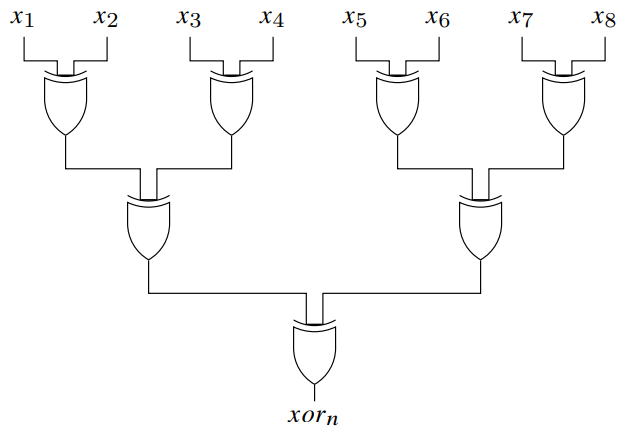
\includegraphics[width=0.5\textwidth, center]{./figures/tree.png}
  \end{solution}
  \begin{solution}
    \begin{itemize}
      \item Für einen balancierten Baum ist Kosten $= \#XOR{-}Gatter = n - 1$ und längster Pfad $= \lceil log(n)\rceil$. Bzw. da vorgegeben, dass $n = 2^k$ gilt, ist auch $log(n)$ korrekt.
    \end{itemize}
  \end{solution}
\end{frame}
